\documentclass[man,floatsintext]{apa6}
\usepackage{lmodern}
\usepackage{amssymb,amsmath}
\usepackage{ifxetex,ifluatex}
\usepackage{fixltx2e} % provides \textsubscript
\ifnum 0\ifxetex 1\fi\ifluatex 1\fi=0 % if pdftex
  \usepackage[T1]{fontenc}
  \usepackage[utf8]{inputenc}
\else % if luatex or xelatex
  \ifxetex
    \usepackage{mathspec}
  \else
    \usepackage{fontspec}
  \fi
  \defaultfontfeatures{Ligatures=TeX,Scale=MatchLowercase}
\fi
% use upquote if available, for straight quotes in verbatim environments
\IfFileExists{upquote.sty}{\usepackage{upquote}}{}
% use microtype if available
\IfFileExists{microtype.sty}{%
\usepackage{microtype}
\UseMicrotypeSet[protrusion]{basicmath} % disable protrusion for tt fonts
}{}
\usepackage{hyperref}
\hypersetup{unicode=true,
            pdftitle={Speakers of diverse languages structure their utterances for efficient communication},
            pdfauthor={Josef Klafka~\& Daniel Yurovsky},
            pdfkeywords={information theory; communication; efficiency; syntax; typology; language development; computational modeling},
            pdfborder={0 0 0},
            breaklinks=true}
\urlstyle{same}  % don't use monospace font for urls
\usepackage{graphicx}
% grffile has become a legacy package: https://ctan.org/pkg/grffile
\IfFileExists{grffile.sty}{%
\usepackage{grffile}
}{}
\makeatletter
\def\maxwidth{\ifdim\Gin@nat@width>\linewidth\linewidth\else\Gin@nat@width\fi}
\def\maxheight{\ifdim\Gin@nat@height>\textheight\textheight\else\Gin@nat@height\fi}
\makeatother
% Scale images if necessary, so that they will not overflow the page
% margins by default, and it is still possible to overwrite the defaults
% using explicit options in \includegraphics[width, height, ...]{}
\setkeys{Gin}{width=\maxwidth,height=\maxheight,keepaspectratio}
\IfFileExists{parskip.sty}{%
\usepackage{parskip}
}{% else
\setlength{\parindent}{0pt}
\setlength{\parskip}{6pt plus 2pt minus 1pt}
}
\setlength{\emergencystretch}{3em}  % prevent overfull lines
\providecommand{\tightlist}{%
  \setlength{\itemsep}{0pt}\setlength{\parskip}{0pt}}
\setcounter{secnumdepth}{0}
% Redefines (sub)paragraphs to behave more like sections
\ifx\paragraph\undefined\else
\let\oldparagraph\paragraph
\renewcommand{\paragraph}[1]{\oldparagraph{#1}\mbox{}}
\fi
\ifx\subparagraph\undefined\else
\let\oldsubparagraph\subparagraph
\renewcommand{\subparagraph}[1]{\oldsubparagraph{#1}\mbox{}}
\fi

%%% Use protect on footnotes to avoid problems with footnotes in titles
\let\rmarkdownfootnote\footnote%
\def\footnote{\protect\rmarkdownfootnote}


  \title{Speakers of diverse languages structure their utterances for efficient communication}
    \author{Josef Klafka\textsuperscript{1}~\& Daniel Yurovsky\textsuperscript{1,2}}
    \date{}
  
\shorttitle{Cross-linguistic information structure}
\affiliation{
\vspace{0.5cm}
\textsuperscript{1} Carnegie Mellon University\\\textsuperscript{2} University of Chicago}
\keywords{information theory; communication; efficiency; syntax; typology; language development; computational modeling}
\usepackage{csquotes}
\usepackage{upgreek}
\captionsetup{font=singlespacing,justification=justified}

\usepackage{longtable}
\usepackage{lscape}
\usepackage{multirow}
\usepackage{tabularx}
\usepackage[flushleft]{threeparttable}
\usepackage{threeparttablex}

\newenvironment{lltable}{\begin{landscape}\begin{center}\begin{ThreePartTable}}{\end{ThreePartTable}\end{center}\end{landscape}}

\makeatletter
\newcommand\LastLTentrywidth{1em}
\newlength\longtablewidth
\setlength{\longtablewidth}{1in}
\newcommand{\getlongtablewidth}{\begingroup \ifcsname LT@\roman{LT@tables}\endcsname \global\longtablewidth=0pt \renewcommand{\LT@entry}[2]{\global\advance\longtablewidth by ##2\relax\gdef\LastLTentrywidth{##2}}\@nameuse{LT@\roman{LT@tables}} \fi \endgroup}


\usepackage{lineno}

\linenumbers

\authornote{

Correspondence concerning this article should be addressed to Josef Klafka, 5000 Forbes Ave. E-mail: \href{mailto:jklafka@andrew.cmu.edu}{\nolinkurl{jklafka@andrew.cmu.edu}}}

\abstract{
What role does communicative efficiency play in how we organize our utterances? In this paper, we present a novel method of examining how much information speakers in a given language communicate in each word, surveying numerous diverse languages. We find that speakers produce frequent and informative words at regular parts of their utterances, depending on language they use. The information distribution for each language is derived in part from the features and genealogy of the language. This robust information distribution characterizes both spoken and written communication, and emerges in children's earliest utterances. However, in real-time communication, in-context word predictability allows listeners to process information at a constant, optimal rate, regardless of the information distribution in the language they understand.


}

\begin{document}
\maketitle

\hypertarget{introduction}{%
\section{Introduction}\label{introduction}}

One of the defining features of human language is its power to transmit information. We use language for a variety of different tasks such as greeting friends, taking notes and signaling group identities. All of these tasks share a common unifying purpose: changing the mental state of the listener or reader (Austin, 1975). Language can naturally be thought of as a code, one that allows speakers to turn their intended meaning into a message that can be transmitted to a listener or reader, and subsequently converted by the listener back into an approximation of the intended meaning (Shannon, 1948).

Beyond its utility as a metaphor, this coding perspective on language is powerful because it allows a framework for rational analysis. If language has evolved to be an optimal code for information transmission, what would be the optimal structure for this code (Anderson \& Milson, 1989)? The optimal code would have to work with two competing pressures: (1) a pressure for listeners to easily and successfully decode messages sent by the speaker, and (2) a pressure for speakers to easily code their messages and transmit them with minimal effort and error. A fundamental constraint on both of these processes is the linear order of spoken language: sounds are produced one at a time and each is unavailable perceptually once it is no longer being produced.

Listeners use a strategic solution which allows them to interpret words in rapid succession: \emph{incremental processing}. People process speech continuously as it arrives, predicting upcoming words and building expectations about the likely meaning of utterances in real-time rather than at their conclusion (Kutas \& Federmeier, 2011; Pickering \& Garrod, 2013; Tanenhaus, Spivey-Knowlton, Eberhard, \& Sedivy, 1995). This solution creates new guidance for speakers: since prediction errors can lead to severe processing costs and difficulty integrating new information on the part of listeners, speakers should seek to minimize prediction errors. However, the cost of producing more predictable utterances is using more words. Thus, the optimal strategy is for speakers seeking to minimize their production costs is to produce utterances that are just at the prediction capacity of listeners without exceeding this capacity (Aylett \& Turk, 2004; Genzel \& Charniak, 2002). In other words, speakers should maintain a constant transmission of information, with the optimal rate of information transfer as close to the listener's fastest decoding rate as possible.

Using information theory, a mathematical framework for formalizing predictability, researchers have tested and confirmed this general prediction of optimal coding across several levels and contexts of language production. For example, Genzel and Charniak (2002) provided a clever indirect test of this hypothesis across sentences in a paragraph. They showed that the predictability of successive sentences, when analyzed in isolation, decreases, as would be expected if readers use prior sentences to predict the content of future sentences. Thus, based on the increasing amount of context, they found that total predictability remains constant. At the level of individual words, Mahowald, Fedorenko, Piantadosi, and Gibson (2013) showed that speakers prefer the shorter versions of words in more predictive contexts, maximizing the amount of information in each word while minimizing the time spent on those words.

Over time, Piantadosi, Tily, and Gibson (2011) showed that more easily predictable words tend to become shorter. Languages evolve so that speakers maximize the amount of information transmitted over the communication channel at every second. Semantic categories of words across languages can evolve to be structured efficiently, maintaining a trade-off between informativeness and complexity in the semantic category, such as kinship terms (Kemp \& Regier, 2012). Languages more generally evolve according to principles of efficient communication: features of the world that are relevant to speakers become part of a language, while irrelevant features are disregarded (Perfors \& Navarro, 2014) and structure in langauge evolves from a trade-off between efficient and learnable encoding on the one hand and an expressive and descriptive lexicon on the other (Kirby, Tamariz, Cornish, \& Smith, 2015).

Other research has suggested that efficient encoding impacts how speakers structure units between words and sentences. The inclusion of complementizers in relative clauses (Jaeger \& Levy, 2007) and the use of contractions (Frank \& Jaeger, 2008) are two situations in sentence formation in which speakers can omit or reduce words to communicate more efficiently and maximize use of the communication channel without exceeding the listener's capacity.

However, despite this literature using the predictive coding model of language, one level has not yet been studied in depth: how speakers structure individual utterances. This level may show the strongest effects of variation between languages, as specific languages have properties that constrain how speakers may form utterances in those languages, such as canonical word order. These properties vary widely from language to language.

Yu, Cong, Liang, and Liu (2016) studied this utterance level in written English sentences using a contextless entropy model based on word frequency. They found a distinctive three-step distribution regardless of sentence length, with little information in the first words of sentences and the most information in the final word. This was surprising, as the distribution they found was robustly different from the linearly increasing trend in sentences from Genzel and Charniak (2002), and also did not resemble the uniform distribution of information that one might expect from a communicative efficiency account, in which each word has approximately equal information close to the channel capacity.

In this paper, we expand on this body of prior work in a number of novel ways. We replicate the results from Yu et al. (2016) with a metric tied to incremental word processing. We find their same distribution of information based on word frequency in English speech as well as in English writing. We extend our metric to include context, and show that the addition of context for each word smoothes out language-specific distributions. We expand the study of information density to the largest set of languages considered so far, and incorporate contextual and typological information into our analysis. Speakers will tend to distribute information in a language constrained but not determined by the morphology, syntax and phonology of that language. Using child speech corpora, we find that as soon as a child starts speaking, they tend to distribute information in their utterances according to the characteristic distribution in their language.

\hypertarget{methods}{%
\section{Methods}\label{methods}}

Shannon (1948) defined information as \enquote{the reduction in uncertainty about one variable given that the value of another variable is known}. We use a metric proposed for the study of information transmission more generally by Shannon and applied to words specifically by Levy (2008): lexical surprisal. This measure defines the information in a word based on the ratio of possible continuations of the sentence after to before the word is seen. Equivalently, we can compute surprisal with the predictability of the word based on previously heard or seen words in its context, as in the formula below. The surprisal of a word is inversely proportional to the predictability of a word, such that less common and less predictable words carry more information.

\[\text{surprisal}(\text{word}) = -\log P(\text{word})\]

The surprisal of a word is also correlated with the processing cost of a word, shown by evidence from e.g.~eye-tracking (Smith \& Levy, 2013) and ERP (Frank, Otten, Galli, \& Vigliocco, 2015) studies. Considered without context, the surprisal of an individual word is inversely proportional to the frequency of that word, so that simply the less often a person has seen a word, the more information that word holds. For example, \enquote{flower} has less information than \enquote{azalea} because \enquote{flower} is much more common than \enquote{azalea}. Though the two words have the same length in number of letters, it is more difficult to process \enquote{azalea} when reading it here than when reading \enquote{flower}. Frequency is intimately tied information content in words, with much of the differences between words frequencies being explained by information content cross-linguistically (Piantadosi et al., 2011).

However, when reading or listening, people don't just consider each word as an isolated linguistic signal. Instead, listeners use the words they have already heard to predict and decode the word they are currently hearing. Following this incremental processing paradigm, we can also condition the surprisal of a word in its context. In the formula below, \(w_i\) denotes the word currently being read or heard, while \(w_{i-1}\) denotes the first word before the current word, \(w_{i-2}\) denotes the second word before the current word, and so on.

\[\text{surprisal}(w_i|w_{i-1}w_{i-2}...) = -log P(w_i|w_{i-1}w_{i-2}...)\]
\[= -log \frac{P(w_i,w_{i-1}w_{i-2},...)}{P(w_{i-1}w_{i-2}...)}\]

When we use a word or two of context in our surprisal calculations, then the set of reasonable final items in our ngrams is greatly restricted. \enquote{Flower} may contain less information than \enquote{azalea} when we consider the words independently of their context, but with context this can be reversed. Flower appears in a variety of contexts, and so the information content of a word like \enquote{flower} in a particular context may be higher than \enquote{azalea}. If you only have azaleas in your garden, then hearing someone say \enquote{in that garden, look at the flowers} may be higher surprisal for you: you expect them to say \enquote{azalea}. This prediction does not require many words for context. For example, in the sentence \enquote{I take my coffee with cream and sugar}, when hearing \enquote{cream and}, a listener might automatically predict \enquote{sugar}, but there are few possible continuations with even the two words \enquote{cream and}. Hearing \enquote{I} restricts the next word to a verb, or possibly an adverb, and since the listener has heard the speaker refer to themselves in the first person singular, their set of possible completions is significantly restricted.

Ideally, we would like to measure the predictability of each word in an utterance using all of the information available to that word. For example, in an utterance of twenty words, we would like to use the previous \(19\) words of context to predict the \(20\)th word. However, we would need to train on a corpus of many trillion word tokens to predict with this amount of context. Regardless of computational constraints, we want to directly compare how predictable each word is regardless of its position in an utterance. We therefore use a simplifying \emph{Markov assumption}: we condition our next predictions on a fixed-size context window instead of all preceding words.

\[\text{surprisal}(w_i|w_{i-1}w_{i-2}...) \approx \text{surprisal}(w_i|w_{i-1}w_{i-2})\]

We train two types of ngram language models independently on a corpus. One of our models is frequency-based: we do not incorporate context into our surprisal calculations. To incorporate context into our models, we train bigram and trigram language models, which incorporate one and two words of context for each processed word, respectively. Although these models may seem to use an inconsequential amount of context when predicting the next word, bigram and trigram models introduce a great deal of improvement over unigram models across tasks (Chen \& Goodman, 1999). Models which incorporate more than two words of context have issues with overfitting to the corpus and only predicting observed sequences, often generalizing poorly.

In our contextual models, we face another issue of overfitting: we only train our model on those utterances which occur in the corpus and test our model on the same utterances. This ignores possible other utterances which the speakers could have produced, e.g.~the words \enquote{I}, \enquote{saw} and \enquote{bears} are in the corpus vocabulary, which a speaker may not have produced as the utterance \enquote{I saw bears} in the corpus but could have produced that utterance. To combat this issue, we use modified Kneser-Ney smoothing as implemented in the KenLM toolkit (Heafield, Pouzyrevsky, Clark, \& Koehn, 2013). Briefly, this smoothing technique discounts all ngram frequency counts, which reduces the impact of rare ngrams on probability calculations, and interpolates lower-order ngrams into the calcuations. These lower-order ngrams are weighted according to the number of distinct contexts they occur as a continuation (e.g. \enquote{Francisco} may be a common word in a corpus, but likely only occurs after \enquote{San} as in \enquote{San Francisco}, so it receives a lower weighting). For a more complete explanation of modified Kneser-Ney smoothing, see Chen and Goodman (1999).

Once we have fitted our language model, we can compute the surprisal of a continuation by simply taking the negative log-probability of that word's ngram probability. To find the average information for a given position in a corpus, we take all utterances of a given length, and for each word position in utterances of that length, we compute the average of the surprisals for all of the non-unique words that occur in that position, conditioned or not conditioned on context. By computing these averages for each word position in an utterance, we compute a low-dimensional approximation to the average distribution of information in the corpus. With the surprisal metric, we base the information contained in each word on how often the word is encountered in its context in the corpus. As long as the corpus is representative of the language or population we study, then the distribution of information is approximated for that language or population as a whole.

The flexibility of the surprisal metric we employ in this paper allows us to calculate the anticipated information for an individual utterance, as most work with the metric has done in the past. Averaging together the surprisal values for a word position within utterances is actually a step further than prior work, and indicates the tendencies speakers gravitate towards instead of examining individual stimuli in psycholinguistic experiments.

The frequency-based surprisal metric gives us an idea of when in their utterances speakers say frequent i.e.~independently information-rich words. The context-based surprisal metric show us how speakers tend to distribute the information in utterances relative to real-time processing in communication. We expect a priori that our frequency-based surprisal curve will be flat. No one part of the sentence will on average have words that are more frequent than another across utterance lengths. Similarly, we expect that there will be a small smoothing effect for our contextual surprisal metric such that the word in each position of an utterance is more predictable than its frequency-based counterpart.

\hypertarget{frequency-based-and-contextual-information-curves-in-written-english-the-british-national-corpus}{%
\section{Frequency-based and contextual information curves in written English: the British National Corpus}\label{frequency-based-and-contextual-information-curves-in-written-english-the-british-national-corpus}}

We first turn to working with written English in the British National Corpus (BNC; Leech, 1992). The BNC is a collection of spoken and written records (90\% written) from the turn of the century, intended to be a representative sample of British English. Using their word entropy metric without context, \#yu2016 found a distinctive three-step distribution for information in written English sentences in the corpus. The first word tended to contain little information. While the middle words of sentences each had more information than the first word, they found a flat and non-increasing rate of information transmission across the middle of sentences. The final word contained the most, though not most, of the information out of any in the sentence, with a noticeable spike in information. They found the same distribution across sentence lengths, from sentences with \(15\) words to sentences with \(45\) words.

We replicate the Yu et al. (2016) result using the surprisal metric in place of the entropy metric. We use the frequency-based or \enquote{contextless} surprisal metric, which determines the average distribution of information based on word frequencies in a corpus. A priori we expect that the frequency-based metric will produce a flat distribution of information across word positions in the BNC. We find the same frequency-based information trajectory as Yu et al.~with little information in the first words of utterances and the most information in the final word, see Figure~\ref{fig:bnc-unigrams}.

\begin{figure}
\centering
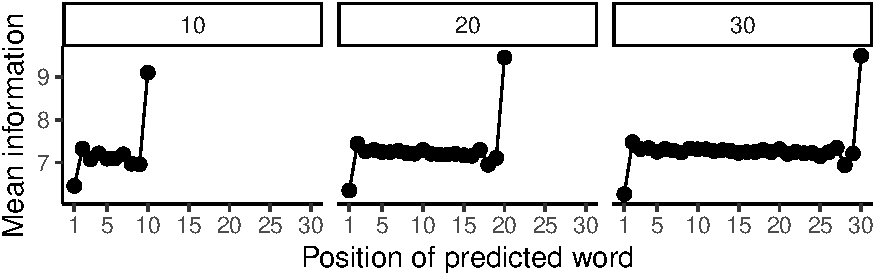
\includegraphics{figs/bnc-unigrams-1.pdf}
\caption{\label{fig:bnc-unigrams}BNC frequency-based information curves}
\end{figure}

We have found a unique average distribution of information that appears to characterize the English language regardless of utterance length. This distribution indicates that in English, the words we speak or write at the beginnings of utterances have little information, while the words we speak or write at the ends of utterances have a lot of information. The words in the middle of utterances have a medial amount of information, without the increasing trend in information from word to word that we might expect from (Genzel \& Charniak, 2002).

What about context? So far we've only discussed the frequency-based metric, considering words on their own without any explicit incorporation of prior context. As previously discussed, listeners decode information and process what they hear incrementally, using prior heard words to ease the comprehension process. We now include two words of context (trigrams) for each word in our measurements. We observe a flattening effect of context across both modalities and all speaker populations. After the first word or two, where the listener does not have access to prior context, then they decode information at a flat and more or less uniform rate. The contextual information curves for the BNC are in Figure \ref{fig:bnc-trigrams}. We also computed bigram curves with one word of context for each prediction: these bigram curves resemble the trigram curves.

\begin{figure}
\centering
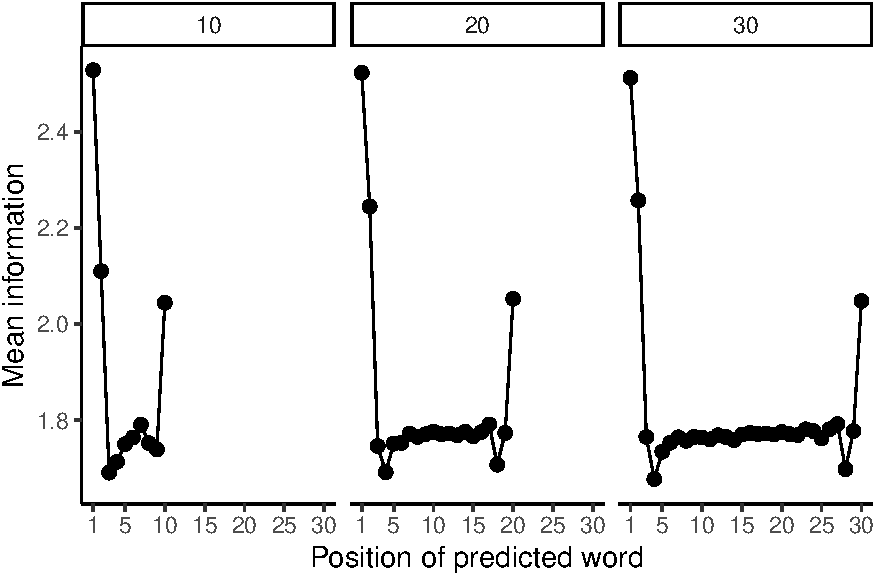
\includegraphics{figs/bnc-trigrams-1.pdf}
\caption{\label{fig:bnc-trigrams}British National Corpus trigram context-based information curves}
\end{figure}

Speakers produce information at a more or less constant rate, avoiding peaks or troughs in their information distribution, except at the beginnings of utterances, where listeners may not have any context to predict what the speaker is going to say. Speakers of English tend towards a characteristic and uneven distribution of word information based on frequencies within their utterances. Their interlocutors, however, once they have a word or two of context, decode information at a more or less constant and optimal rate.

\hypertarget{frequency-based-and-contextual-information-curves-in-spoken-english-the-british-national-corpus}{%
\section{Frequency-based and contextual information curves in spoken English: the British National Corpus}\label{frequency-based-and-contextual-information-curves-in-spoken-english-the-british-national-corpus}}

We found that English speakers and writers used the same robust and distinctive distribution of information within each utterance, regardless of the number of words in their utterances. To determine if this distribution truly characterizes all speakers of the English language as a whole, we wanted to examine speech from English-speaking children who are producing their very first multi-word utterances. We hypothesize the three-step distribution of information we found for English will characterize child speech and child-directed speech. This approach also allows us to analyze parent speech to children, to examine speech more generally and understand if English speech gives rise to the same information distribution as English writing.

We use the North American English collection from CHILDES (MacWhinney, 2000), which consists of about 2.6 million utterances from 522 children and their parents across 49 corpora. We obtained this collection using the childesr frontend to the childes-db database (Sanchez et al., 2019). The utterances in the Providence corpus are on average significantly shorter than those in the BNC; over 95\% of the utterances in the North American English collection are \(10\) words or fewer. Unlike the written BNC, which we split by sentence, we split our CHILDES corpus by conversational turns and pauses using the built-in utterance breaks for each corpus.

We observe the same distinctive distribution of information for parents and children in the child speech corpus as we did for adults in the BNC. The distribution of information we find at the level of individual words in English, therefore, characterizes the English language as a whole and not only adult utterances, not only written utterances. See \ref{fig:eng-unigrams}.

\begin{figure}
\centering
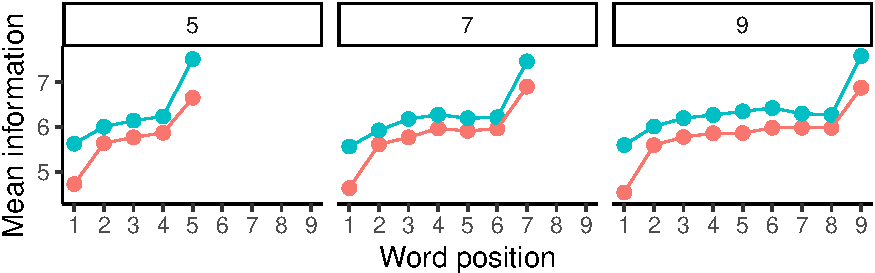
\includegraphics{figs/eng-unigrams-1.pdf}
\caption{\label{fig:eng-unigrams}North American English frequency-based information curves. Lines around each point indicate 95\% confidence intervals computed with non-parametric bootstrap}
\end{figure}

What about predictive processing in child-directed speech and child speech? When incorporating one or two words of predictive context, we observe the same trend as in the BNC. Beyond the first couple of words, once your interlocutor has enough context to predict with some accuracy what you will say next, then you decode information from their speech stream at a constant and optimal rate. This applies to parents and children speaking to one another, as well as adults speaking and writing to one another. See \ref{fig:eng-trigrams}.

\begin{figure}
\centering
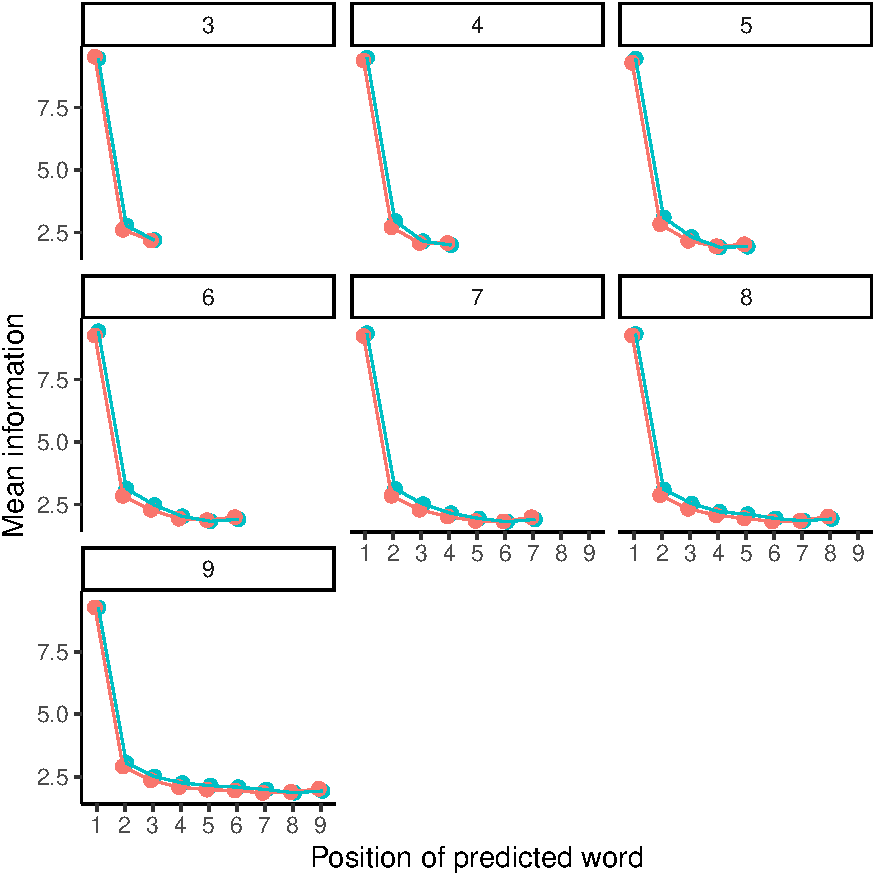
\includegraphics{figs/eng-trigrams-1.pdf}
\caption{\label{fig:eng-trigrams}North American English context-based information curves. Lines around each point indicate 95\% confidence intervals computed with non-parametric bootstrap}
\end{figure}

\hypertarget{frequency-based-and-contextual-information-curves-across-languages-a-qualitative-analysis}{%
\section{Frequency-based and contextual information curves across languages: a qualitative analysis}\label{frequency-based-and-contextual-information-curves-across-languages-a-qualitative-analysis}}

So far, we have only looked at the distribution of information in words in English, both with and without context. We have examined child speech and child-directed speech at a variety of ages, as well as writing samples selected to be representative of British English as a whole. But this only captures the picture for English.

We now turn to a small number of typologically diverse languages, and conduct the same analysis, using monolingual adult-child speech corpora from CHILDES (MacWhinney, 2000) to compare the results from these languages directly to our results from English. We use corpora for Spanish, German, French, Mandarin Chinese and Japanese. Similar to our English child speech collection, all of the language collections consist mainly of shorter utterances: most utterances in the corpora are under 10 words long. Mandarin and Japanese are not natively written using the Latin alphabet, and moreover words are not segmented in their native scripts. Instead of the native scripts, we use transliterations from the corpus for each of the Mandarin and Japanese utterances into pinyin for Mandarin and romanji for Japanese. In these transliterations, words are previously segmented.

We observe a distinct and characteristic frequency-based information trajectory for each language, robust across each utterance length. We see the same distribution of information for both parents and children. The parent often has more information on average at each word position in their utterances. This is an effect of the surprisal metric: parents speak more utterances than their children in most of the corpora, which inflates the number of tokens they use and increases the surprisal of hearing a rare word. We include the frequency-based information curve from the North American English CHILDES collection for comparison. See Figure~\ref{fig:childes-unigrams}

\begin{figure}
\centering
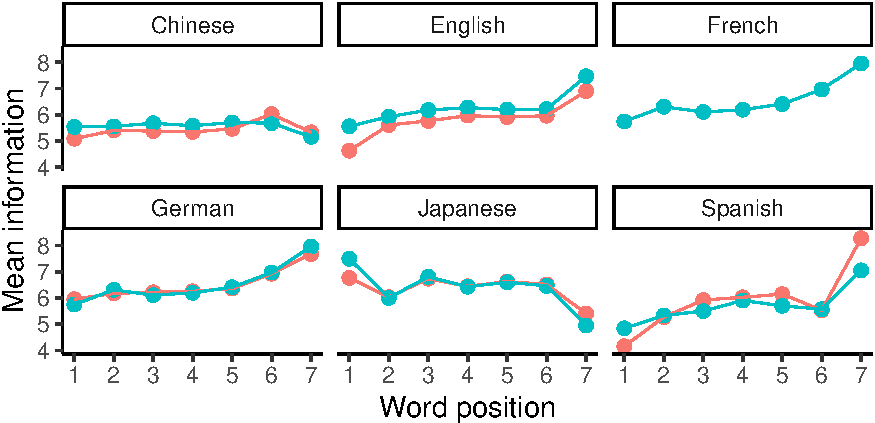
\includegraphics{figs/childes-unigrams-1.pdf}
\caption{\label{fig:childes-unigrams}CHILDES frequency-based information curves}
\end{figure}

English, Spanish, French and German feature similar information curve shapes, with slight variations. The German information curve features lower information for longer towards the beginnings of utterances, possibly due to the grammatical restriction that the second word in German utterances must be a verb (V2). Spanish features a larger spike in the amount of information in the final word of utterances. For Japanese and Mandarin, we observe completely different frequency-based information curve trajectories. The Japanese frequency-based information curve trajectory begins high and finishes low, the mirror image of the German and Romance language information curves. The Mandarin curve begins low and finishes low, but features high information in the middle of utterances. We hypothesize this may be due to Japanese and Mandarin speakers typically ending their utterances with particles, which are common and thus contain little information on their own.

For the rigram information curves, we see the same contextual smoothing effect as in English. While the frequency-based information curves may depend based on the language, the contextual information curves show the same trajectory cross-linguistically. Using more than two words of context is difficult for parent-child speech corpora because the utterances are so short on average (less than \(10\) words). Based on our results from the CHILDES collections, we hypothesize that the frequency-based information curves may vary based on the genealogy and typology of the languages in question. However, this does not extend to the information curves with two words of context in particular, where all languages we have seen so far are characterized by the same information distribution. See Figure~\ref{fig:childes-trigrams}.

\begin{figure}
\centering
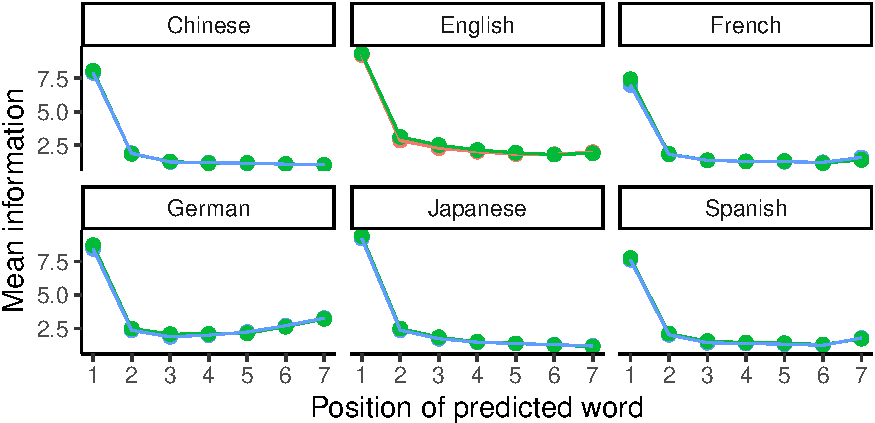
\includegraphics{figs/childes-trigrams-1.pdf}
\caption{\label{fig:childes-trigrams}CHILDES trigram context-based information curves}
\end{figure}

\hypertarget{language-structures-and-large-scale-data-analysis-methods}{%
\section{Language structures and large-scale data analysis: methods}\label{language-structures-and-large-scale-data-analysis-methods}}

To make a claim about how languages on a larger scale, we need to use larger corpora and a much larger number of languages. We pulled corpora for \(159\) diverse languages from Wikipedia, each of which had at least \(10,000\) articles on the knowledge base. We split each article into sentences; the variance in sentence lengths for Wikipedia was significantly larger than for the CHILDES corpora we used in the previous section. Most sentences in Wikipedia contained between \(10\) and \(30\) words, unlike the CHILDES corpora which mainly contained utterances with under \(10\) words. We excluded the small fraction of utterances with more than \(50\) words since they were small in number and, from manual inspection, uncharacteristic of typical written sentences.

How do we quantitatively analyze information curves for more than \(40\) difference sentence lengths for each language, adding up to several thousand information curves total? We used two different strategies, which yielded identical results upon analysis. Each strategy gave us a five-dimensional vector for each language in a Wikipedia \enquote{slope space}. For the first strategy, we split each sentence length by number of words into fifths, and computed surprisal values for the closest word position to each quintile. We then computed the slopes between the surprisal values at neighboring quintiles, yielding five slope values for each curve. For the second strategy, we split each sentence length by number of words into sections based on those areas of the information curves that had seemed most important in our CHILDES analysis: between the first and second word; between the second and third word; between the third word and third-to-last word; between the third-to-last word and the second to last word; and between the second-to-last word and the last word. We then computed surprisal values at each of these positions, and computed slopes between the surprisal values at each section, giving us another five slope values for each language summarizing the information curves. We computed frequency-based and trigram contextual information curves for each language, using the aggregation strategies described above.

We include illustrations of these two strategies using the frequency-based curve from the British National Corpus in Figure \ref{fig:treatments}

\begin{figure}
\centering
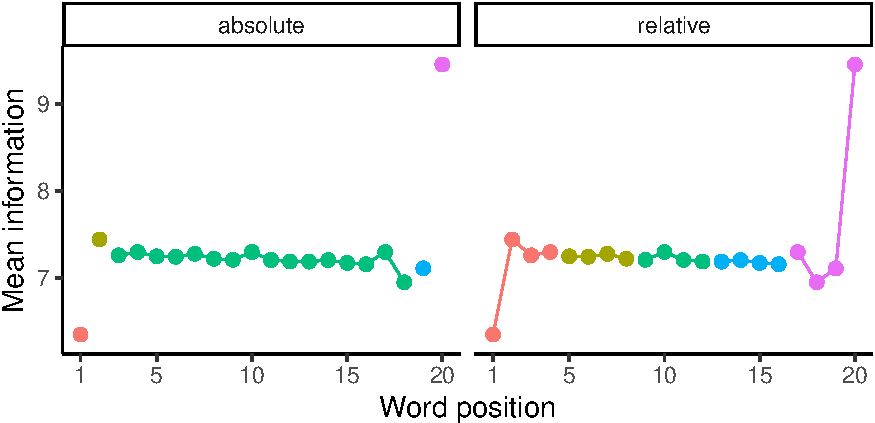
\includegraphics{figs/treatments-1.pdf}
\caption{\label{fig:treatments}Illustration of slope treatments for Wikipedia information curves: relative on top and absolute on bottom}
\end{figure}

To more rigorously described the typological differences between languages, we used data from the World Atlas of Language Structures (WALS; Dryer \& Haspelmath, 2013). The WALS database has data for \(144\) typological features in \(2569\) languages from across the world. These features describe aspects of morphology, syntax, phonology, etymology and semantics--in short the features describe the structures in each language. As WALS is a compiled database from dozens of papers from different authors, most of the features and languages are fairly sparse. Even limiting ourselves to the \(159\) language corpora we pulled from Wikipedia and \(122\) features from WALS, there are nearly \(20000\) individual possible data values, fewer than half of which were already computed for those languages in the WALS database.

To fill in the missing data for the features we selected using statistical imputation, we used Multiple Imputation Multiple Correspondence Analysis (MIMCA; Audigier, Husson, \& Josse, 2017). MIMCA begins with mean imputation, converts the categorical WALS features into a numerical contingency table with dummy coding, then repeatedly performs principle components analysis and reconstructs the contingency table. Our final result from the MIMCA algorithm was a fully imputed table with \(122\) feature values for each language.

However, the WALS features describe specific structural differences between languages, while our surprisal metric is word-based. To target lexical differences between languages, we computed the average normalized Levenshtein distance (LDN; Holman et al., 2008) over the \(40\) item Swadesh list (Swadesh, 1955), retrieved from the ASJP database (Wichmann et al., 2016). The Swadesh list is designed to include near-universal words that target basic cognitive concepts, and are useful in determining the genealogical similarities and differences between languages. The results of classifying languages using the Swadesh list and LDN are correlated with those using WALS features, but the Swadesh list and LDN do not suffer from the same sparsity problem as WALS (Holman et al., 2008).

\hypertarget{language-structures-and-large-scale-data-analysis-results}{%
\section{Language structures and large-scale data analysis: results}\label{language-structures-and-large-scale-data-analysis-results}}

We ran a hierarchical clustering algorithm on the frequency-based information curves using the hclust package from the R stats core library (Team \& others, 2013). We used the complete linkage algorithm for hierarchical clustering, with distances between information curves between languages computed using cosine distance between their embeddings in the slope space. The complete linkage algorithm at every step pairs each language or cluster of languages with its closest neighboring language or cluster. A sample from the dendrogram is shown in Figure~\ref{fig:dendro}. From a quick glance, the unigram information curves appear to reproduce some of the genealogical relationships between languages, although the dendrogram does not exactly replicate language genealogy for all \(159\) languages. This suggests using a first-pass quantitative method that the information curves do correspond in some measure to language families, but language families do not explain all of the variation and relationships between frequency-based information curves.

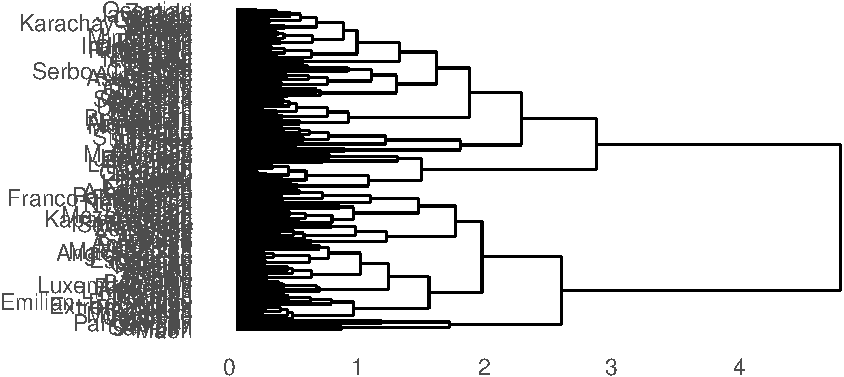
\includegraphics{figs/dendro-1.pdf}

A sample of the contextual information curves (computed using two words of context) are plotted in Figure~\ref{fig:wiki-trigrams}, and all contextual information curves for the languages we used follow the same pattern. The first few words in utterances for each language are surprising, but after even two words of predictive context for each word, the amount of information in each word flattens. Regardless of language, speakers produce information at a constant, optimal rate.

\begin{figure}
\centering
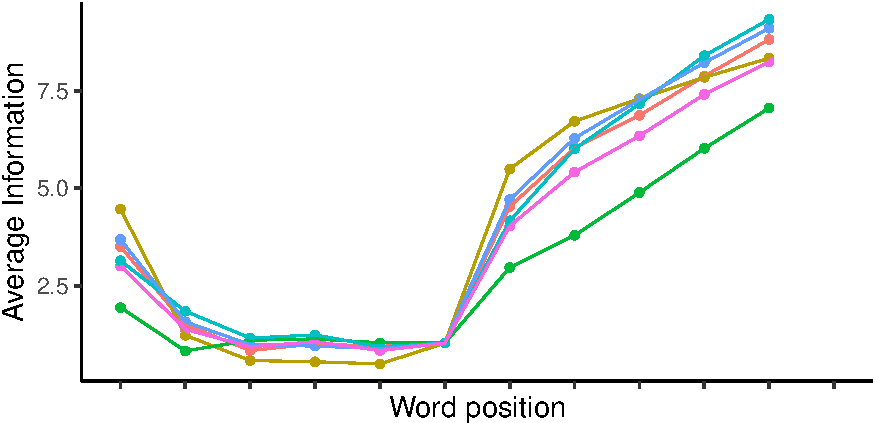
\includegraphics{figs/wiki-trigrams-1.pdf}
\caption{\label{fig:wiki-trigrams}Some trigram information curves from the Wikipedia data}
\end{figure}

For our first quantitative analysis, we examined the effects of individual typological features on the shapes of the unigram information curves. We ran logistic regressions using the lme4 package in R (Bates, Mächler, Bolker, \& Walker, 2014), checking whether the cosine distance between two languages' embeddings in the slope space played a role in determining if those two languages had the same value for a given WALS feature. Individual WALS features do not necessarily have ordinal values. Some, such as the \enquote{Number of Cases} feature, are easy to quantify and order. Others are more difficult. For example, how does one order \enquote{relative clauses appear after the nouns they modify}, \enquote{relative clauses appear before the nouns they modify} and \enquote{free order of relative clauses and nouns}? We chose the identify relation to avoid deciding on the basis of individual features. We found that 100 out of the 122 features from WALS we examined were statistically significant (p \textless{} .001) in determining whether two languages had the same frequency-based information curve shape. The results for some important features are in Figure~\ref{fig:linear-models}.

\begin{figure}
\centering
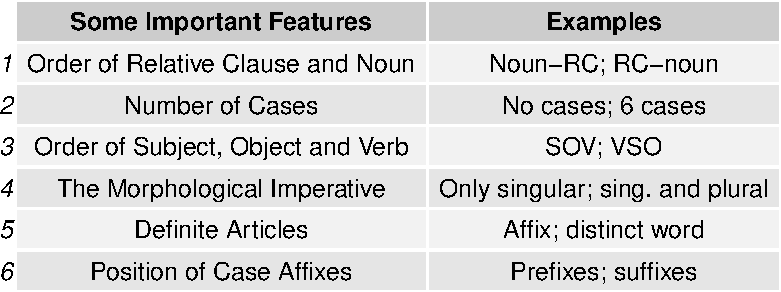
\includegraphics{figs/linear-models-1.pdf}
\caption{\label{fig:linear-models}Some linear model results from Wikipedia and WALS features}
\end{figure}

We next compared how the cosine distance between two languages related to how many WALS features they had in common. \(r^2\) value is \(.005734\), which suggests that in aggregate there is not a correlation between how many WALS features languages have in common and the similarity of their frequency-based information curves. Figure \ref{fig:cosine-wals} displays the results. This result is surprising based on the significance of many WALS features in predicting the shapes of the frequency-based information curves, and we return to this result in the general discussion.

\begin{figure}
\centering
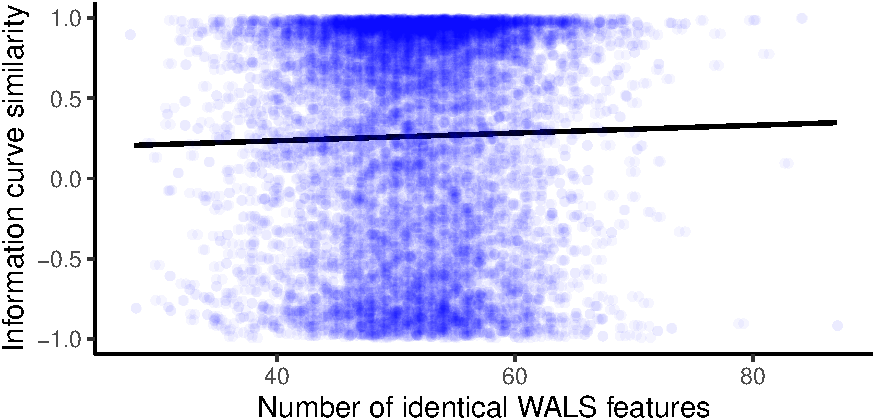
\includegraphics{figs/cosine-wals-1.pdf}
\caption{\label{fig:cosine-wals}wals features vs cosine similarity}
\end{figure}

For lexical features, we see a stronger correlation between the similarity of two languages in terms of their average LDN and the cosine distance between their information curves. Figure \ref{fig:cosine-ldn}. We see a higher \(r^2\) value here of \(.026\), indicating that there is more correspondence between a language's lexical similarity to another language and their similarity in information curves. From these typological and lexical investigations, we conclude that the shape of a language's frequency-based information curve covaries with its typological and lexical similarity to other languages. However, most of the variation in frequency-based information curve shapes is not explained by typological properties in language.

\begin{figure}
\centering
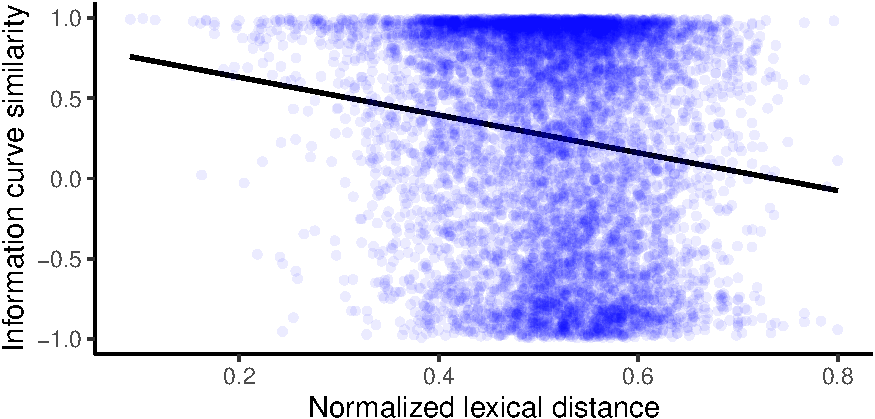
\includegraphics{figs/cosine-ldn-1.pdf}
\caption{\label{fig:cosine-ldn}ldn features vs cosine similarity}
\end{figure}

\hypertarget{discussion}{%
\section{Discussion}\label{discussion}}

By considering the distribution of information at the level of utterances and sentences, we join together the information-theoretic work focusing on sub-word units and words, and that focusing on paragraphs. In doing so, we show that frequency and context-based metrics complement one another in studying efficiency and information in language. We directly link linguistic efficiency in a language to the genealogy and properties of that language. We provide evidence for a novel linguistic universal: low processing cost for listeners beyond the first words in utterances, driven by high average word predictability in conversation. With consideration to language acquisiton, we observe that children tend to distribute information in their utterances according to the their language's frequency-based information curve as soon as they form multi-word utterances.

Throughout this work we have averaged the surprisal values at each position. Averaging removes variation, which in turn may obscure trends in the data. As discussed in the methods section, the surprisal metric has historically been used for calculating the information and processing cost for individual utterances, and our use of the metric here is actually a step forward rather than a step back. Future work can investigate variation in how speakers distribute information in individual utterances.

The WALS database we used to investigate typological variation in the information curves is overall sparse. We imputed well over \(50\%\) of the WALS features for most of our \(159\) languages, although all of the languages had at least \(20\) features evaluated in WALS. A large part of this is due to WALS being a collection of a number of different studies, instead of a systematic effort to catalogue variation across the world's languages. Additionally, WALS features are meant to describe specific microvariations in languages, not to provide a comprehensive typological representation of each language compared to each other language. This may be why the Swadesh list provided a higher correlation for describing the differences in information curves: Swadesh (1955) intended the list to allow researchers to more comprehensively compared and constrast lexical differences between languages. For our Wikipedia analysis, we also reduce all of a language's variation down to a five-dimensional vector. These information curve representations show a surprising amount of variation despite the degree of compression.

\newpage

\hypertarget{references}{%
\section{References}\label{references}}

\begingroup
\setlength{\parindent}{-0.5in}
\setlength{\leftskip}{0.5in}

\hypertarget{refs}{}
\leavevmode\hypertarget{ref-anderson1989}{}%
Anderson, J. R., \& Milson, R. (1989). Human memory: An adaptive perspective. \emph{Psychological Review}, \emph{96}(4), 703.

\leavevmode\hypertarget{ref-audigier2017}{}%
Audigier, V., Husson, F., \& Josse, J. (2017). MIMCA: Multiple imputation for categorical variables with multiple correspondence analysis. \emph{Statistics and Computing}, \emph{27}(2), 501--518.

\leavevmode\hypertarget{ref-austin1975}{}%
Austin, J. L. (1975). \emph{How to do things with words}. Oxford university press.

\leavevmode\hypertarget{ref-aylett2004}{}%
Aylett, M., \& Turk, A. (2004). The smooth signal redundancy hypothesis: A functional explanation for relationships between redundancy, prosodic prominence, and duration in spontaneous speech. \emph{Language and Speech}, \emph{47}(1), 31--56.

\leavevmode\hypertarget{ref-bates2014}{}%
Bates, D., Mächler, M., Bolker, B., \& Walker, S. (2014). Fitting linear mixed-effects models using lme4. \emph{arXiv Preprint arXiv:1406.5823}.

\leavevmode\hypertarget{ref-chen1999empirical}{}%
Chen, S. F., \& Goodman, J. (1999). An empirical study of smoothing techniques for language modeling. \emph{Computer Speech \& Language}, \emph{13}(4), 359--394.

\leavevmode\hypertarget{ref-wals}{}%
Dryer, M. S., \& Haspelmath, M. (Eds.). (2013). \emph{WALS online}. Leipzig: Max Planck Institute for Evolutionary Anthropology. Retrieved from \url{https://wals.info/}

\leavevmode\hypertarget{ref-frank2008}{}%
Frank, A. F., \& Jaeger, T. F. (2008). Speaking rationally: Uniform information density as an optimal strategy for language production. In \emph{Proceedings of the annual meeting of the cognitive science society} (Vol. 30).

\leavevmode\hypertarget{ref-frank2015}{}%
Frank, S. L., Otten, L. J., Galli, G., \& Vigliocco, G. (2015). The erp response to the amount of information conveyed by words in sentences. \emph{Brain and Language}, \emph{140}, 1--11.

\leavevmode\hypertarget{ref-genzel2002}{}%
Genzel, D., \& Charniak, E. (2002). Entropy rate constancy in text. In \emph{Proceedings of the 40th annual meeting of the association for computational linguistics} (pp. 199--206).

\leavevmode\hypertarget{ref-heafield2013scalable}{}%
Heafield, K., Pouzyrevsky, I., Clark, J. H., \& Koehn, P. (2013). Scalable modified kneser-ney language model estimation. In \emph{Proceedings of the 51st annual meeting of the association for computational linguistics (volume 2: Short papers)} (pp. 690--696).

\leavevmode\hypertarget{ref-holman2008}{}%
Holman, E. W., Wichmann, S., Brown, C. H., Velupillai, V., Müller, A., Bakker, D., \& others. (2008). Advances in automated language classification. \emph{Quantitative Investigations in Theoretical Linguistics}, 40--43.

\leavevmode\hypertarget{ref-jaeger2007}{}%
Jaeger, T. F., \& Levy, R. P. (2007). Speakers optimize information density through syntactic reduction. In \emph{Advances in neural information processing systems} (pp. 849--856).

\leavevmode\hypertarget{ref-kemp2012kinship}{}%
Kemp, C., \& Regier, T. (2012). Kinship categories across languages reflect general communicative principles. \emph{Science}, \emph{336}(6084), 1049--1054.

\leavevmode\hypertarget{ref-kirby2015compression}{}%
Kirby, S., Tamariz, M., Cornish, H., \& Smith, K. (2015). Compression and communication in the cultural evolution of linguistic structure. \emph{Cognition}, \emph{141}, 87--102.

\leavevmode\hypertarget{ref-kutas2011}{}%
Kutas, M., \& Federmeier, K. D. (2011). Thirty years and counting: Finding meaning in the n400 component of the event-related brain potential (erp). \emph{Annual Review of Psychology}, \emph{62}, 621--647.

\leavevmode\hypertarget{ref-leech1992}{}%
Leech, G. N. (1992). 100 million words of english: The british national corpus (bnc).

\leavevmode\hypertarget{ref-levy2008}{}%
Levy, R. (2008). Expectation-based syntactic comprehension. \emph{Cognition}, \emph{106}(3), 1126--1177.

\leavevmode\hypertarget{ref-macwhinney2000}{}%
MacWhinney, B. (2000). \emph{The childes project: The database} (Vol. 2). Psychology Press.

\leavevmode\hypertarget{ref-mahowald2013}{}%
Mahowald, K., Fedorenko, E., Piantadosi, S. T., \& Gibson, E. (2013). Info/information theory: Speakers choose shorter words in predictive contexts. \emph{Cognition}, \emph{126}(2), 313--318.

\leavevmode\hypertarget{ref-perfors2014language}{}%
Perfors, A., \& Navarro, D. J. (2014). Language evolution can be shaped by the structure of the world. \emph{Cognitive Science}, \emph{38}(4), 775--793.

\leavevmode\hypertarget{ref-piantadosi2011}{}%
Piantadosi, S. T., Tily, H., \& Gibson, E. (2011). Word lengths are optimized for efficient communication. \emph{Proceedings of the National Academy of Sciences}, \emph{108}(9), 3526--3529.

\leavevmode\hypertarget{ref-pickering2013}{}%
Pickering, M. J., \& Garrod, S. (2013). An integrated theory of language production and comprehension. \emph{Behavioral and Brain Sciences}, \emph{36}(4), 329--347.

\leavevmode\hypertarget{ref-sanchez2019}{}%
Sanchez, A., Meylan, S. C., Braginsky, M., MacDonald, K. E., Yurovsky, D., \& Frank, M. C. (2019). Childes-db: A flexible and reproducible interface to the child language data exchange system. \emph{Behavior Research Methods}, \emph{51}(4), 1928--1941.

\leavevmode\hypertarget{ref-shannon1948}{}%
Shannon, C. E. (1948). A mathematical theory of communication. \emph{Bell System Technical Journal}, \emph{27}(3), 379--423.

\leavevmode\hypertarget{ref-smith2013}{}%
Smith, N. J., \& Levy, R. (2013). The effect of word predictability on reading time is logarithmic. \emph{Cognition}, \emph{128}(3), 302--319.

\leavevmode\hypertarget{ref-swadesh1955}{}%
Swadesh, M. (1955). Towards greater accuracy in lexicostatistic dating. \emph{International Journal of American Linguistics}, \emph{21}(2), 121--137.

\leavevmode\hypertarget{ref-tanenhaus1995}{}%
Tanenhaus, M. K., Spivey-Knowlton, M. J., Eberhard, K. M., \& Sedivy, J. C. (1995). Integration of visual and linguistic information in spoken language comprehension. \emph{Science}, \emph{268}(5217), 1632--1634.

\leavevmode\hypertarget{ref-team2013}{}%
Team, R. C., \& others. (2013). R: A language and environment for statistical computing.

\leavevmode\hypertarget{ref-wichmann2016}{}%
Wichmann, S., Müller, A., Wett, A., Velupillai, V., Bischoffberger, J., Brown, C. H., \ldots{} others. (2016). The asjp database. \emph{Max Planck Institute for the Science of Human History, Jena}.

\leavevmode\hypertarget{ref-yu2016}{}%
Yu, S., Cong, J., Liang, J., \& Liu, H. (2016). The distribution of information content in english sentences. \emph{arXiv Preprint arXiv:1609.07681}.

\endgroup


\end{document}
